%%%%%%%%%%%%%%%%%%%%%%%%%%%%%%%%%%%%%%%%%
% Wenneker Assignment
% LaTeX Template
% Version 2.0 (12/1/2019)
%
% This template originates from:
% http://www.LaTeXTemplates.com
%
% Authors:
% Vel (vel@LaTeXTemplates.com)
% Frits Wenneker
%
% License:
% CC BY-NC-SA 3.0 (http://creativecommons.org/licenses/by-nc-sa/3.0/)
% 
%%%%%%%%%%%%%%%%%%%%%%%%%%%%%%%%%%%%%%%%%

%----------------------------------------------------------------------------------------
%	PACKAGES AND OTHER DOCUMENT CONFIGURATIONS
%----------------------------------------------------------------------------------------

\documentclass[11pt]{scrartcl} % Font size

%%%%%%%%%%%%%%%%%%%%%%%%%%%%%%%%%%%%%%%%%
% Wenneker Assignment
% Structure Specification File
% Version 2.0 (12/1/2019)
%
% This template originates from:
% http://www.LaTeXTemplates.com
%
% Authors:
% Vel (vel@LaTeXTemplates.com)
% Frits Wenneker
%
% License:
% CC BY-NC-SA 3.0 (http://creativecommons.org/licenses/by-nc-sa/3.0/)
% 
%%%%%%%%%%%%%%%%%%%%%%%%%%%%%%%%%%%%%%%%%

%----------------------------------------------------------------------------------------
%	PACKAGES AND OTHER DOCUMENT CONFIGURATIONS
%----------------------------------------------------------------------------------------

\usepackage{amsmath, amsfonts, amsthm} % Math packages

\usepackage{listings} % Code listings, with syntax highlighting

\usepackage[english]{babel} % English language hyphenation

\usepackage{graphicx} % Required for inserting images
\graphicspath{{Figures/}{./}} % Specifies where to look for included images (trailing slash required)

\usepackage{booktabs} % Required for better horizontal rules in tables

\numberwithin{equation}{section} % Number equations within sections (i.e. 1.1, 1.2, 2.1, 2.2 instead of 1, 2, 3, 4)
\numberwithin{figure}{section} % Number figures within sections (i.e. 1.1, 1.2, 2.1, 2.2 instead of 1, 2, 3, 4)
\numberwithin{table}{section} % Number tables within sections (i.e. 1.1, 1.2, 2.1, 2.2 instead of 1, 2, 3, 4)

\setlength\parindent{0pt} % Removes all indentation from paragraphs

\usepackage{enumitem} % Required for list customisation
\setlist{noitemsep} % No spacing between list items

%----------------------------------------------------------------------------------------
%	DOCUMENT MARGINS
%----------------------------------------------------------------------------------------

\usepackage{geometry} % Required for adjusting page dimensions and margins

\geometry{
	paper=a4paper, % Paper size, change to letterpaper for US letter size
	top=2cm, % Top margin
	bottom=2cm, % Bottom margin
	left=2cm, % Left margin
	right=2cm, % Right margin
	headheight=0.75cm, % Header height
	footskip=1.5cm, % Space from the bottom margin to the baseline of the footer
	headsep=0.75cm, % Space from the top margin to the baseline of the header
	%showframe, % Uncomment to show how the type block is set on the page
}

%----------------------------------------------------------------------------------------
%	FONTS
%----------------------------------------------------------------------------------------

\usepackage[utf8]{inputenc} % Required for inputting international characters
\usepackage[T1]{fontenc} % Use 8-bit encoding

\usepackage{fourier} % Use the Adobe Utopia font for the document

%----------------------------------------------------------------------------------------
%	SECTION TITLES
%----------------------------------------------------------------------------------------

\usepackage{sectsty} % Allows customising section commands

\sectionfont{\vspace{6pt}\centering\normalfont\scshape} % \section{} styling
\subsectionfont{\normalfont\bfseries} % \subsection{} styling
\subsubsectionfont{\normalfont\itshape} % \subsubsection{} styling
\paragraphfont{\normalfont\scshape} % \paragraph{} styling

%----------------------------------------------------------------------------------------
%	HEADERS AND FOOTERS
%----------------------------------------------------------------------------------------

\usepackage{scrlayer-scrpage} % Required for customising headers and footers

\ohead*{} % Right header
\ihead*{} % Left header
\chead*{} % Centre header

\ofoot*{} % Right footer
\ifoot*{} % Left footer
\cfoot*{\pagemark} % Centre footer
 % Include the file specifying the document structure and custom commands

%----------------------------------------------------------------------------------------
%	TITLE SECTION
%----------------------------------------------------------------------------------------

\usepackage{float}
\title{	
	Homework 2
}

\author{Yuan Jiahao 2019010070} % Your name

\date{\normalsize\today} % Today's date (\today) or a custom date

\begin{document}

\maketitle % Print the title

\section{Todo}

Run the given quicksort and mergesort serial codes, find the opportunity to use OpenMP
task parallel, add OpenMP instruction statement \# pragma omp task to parallelize it, and verify
the result correctness, test performance, write them in the report.

Call the qsort() function. Test the code of the given qsort() function in the C standard
library, compare the performance with your own parallel code, and write it in the report.

\section{Hardware Environment of the Machine }
The machine's CPU is Intel Core I7-8700,3.2GHz with 6 cores and 12 threads.And the memory is 32GB,DDR4,3200MHz.And the system is windows subsystem for linux,Ubuntu 20.04.

\section{Results}
	\subsection{given quicksort and mergesort serial codes' performance under different threads }
	\subsubsection{performance under single thread }
	\begin{figure}[H]
		\centering
		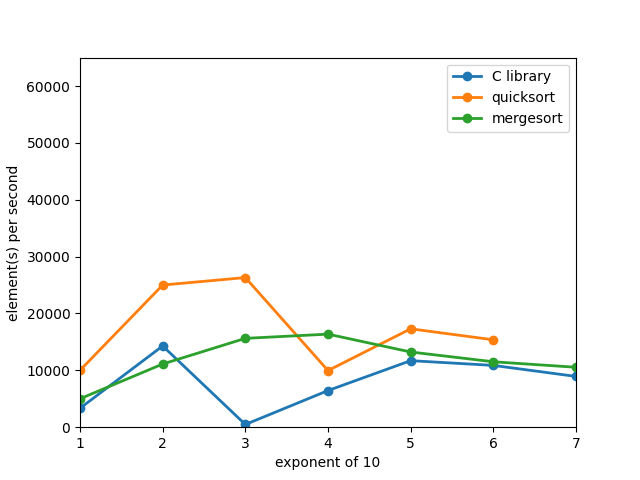
\includegraphics[width=0.8\textwidth]{oricsvtime.png}
		\caption{performance under 1 threads}
		\label{f1}
	\end{figure}
	It's obvious that when the to sort array is completely random and the length of array is not such great,quicksort is the fastest algorithm than the others.However,the chart of quicksort ends before the length comes to $10^7$,why?

	A conjecture is that when the length goes too big,the recursion becomes too deep and cause stack overflow.
	\subsubsection{performance under several threads }
	\begin{figure}[H]
		\centering
		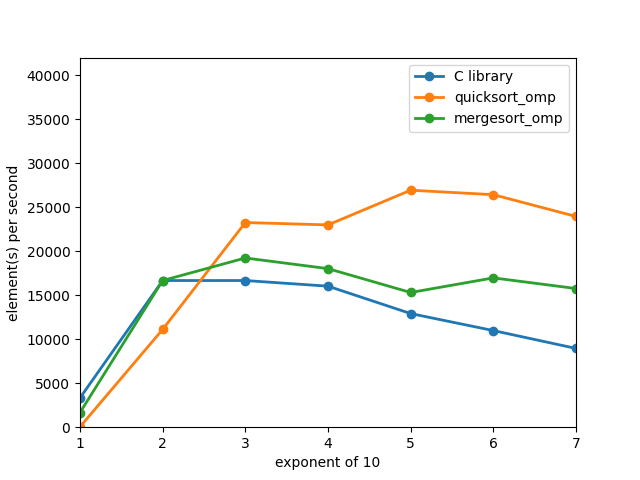
\includegraphics[width=0.8\textwidth]{omp4.csvtime.png}
		\caption{performance under 4 threads}
		\label{}
	\end{figure}
	\begin{figure}[H]
		\centering
		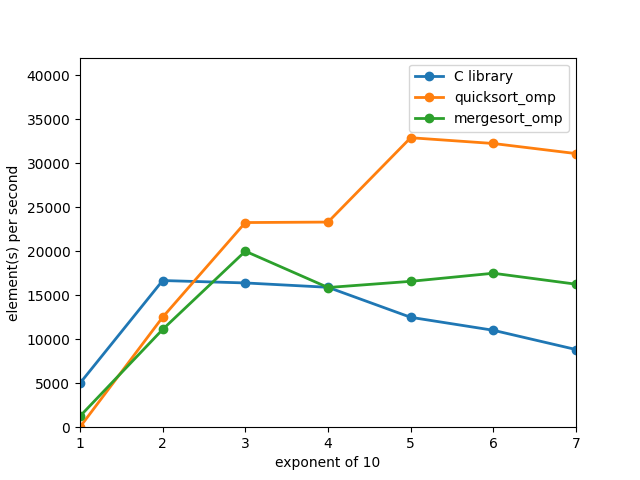
\includegraphics[width=0.8\textwidth]{omp8.csvtime.png}
		\caption{performance under 8 threads}
		\label{}
	\end{figure}
	\begin{figure}[H]
		\centering
		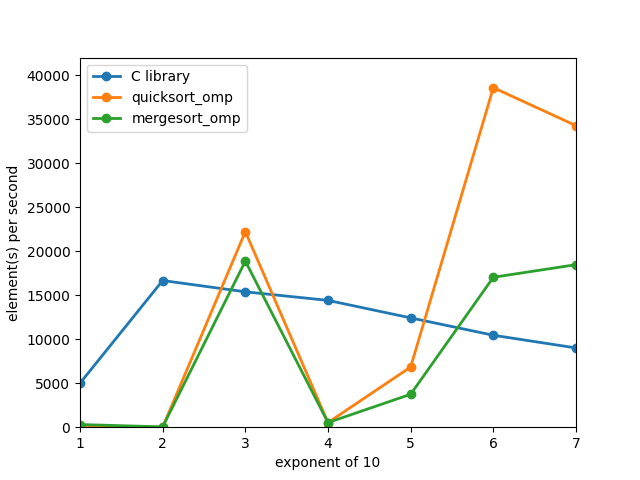
\includegraphics[width=0.8\textwidth]{omp12.csvtime.png}
		\caption{performance under 12 threads}
		\label{}
	\end{figure}
	As the three figures above,we find it's always the quicksort algorithm performs worse than others at first and better when the length of array is large.

	Here we put all of them and my optimized code(which will be discussed later) in one figure to figure out some much more common conclusions.
	\begin{figure}[H]
		\centering
		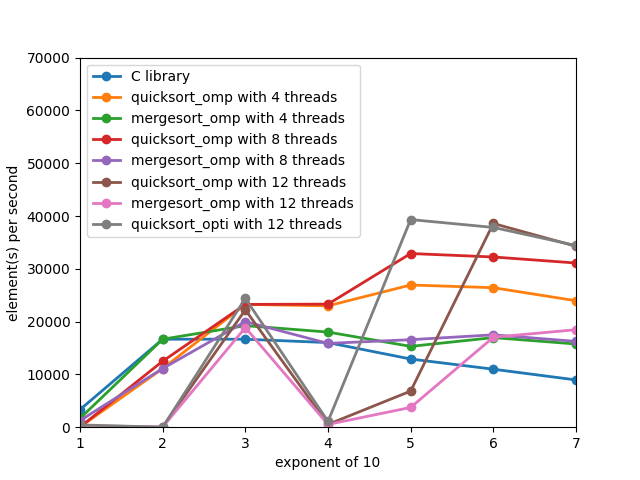
\includegraphics[width=0.8\textwidth]{threads.png}
		\caption{all data in one figure}
		\label{}
	\end{figure}
	One interesting thing is that the merge sort algorithm didn't performs better as the threads add,even became worse at some cases.On the contract,the quicksort's performance get better as the threads add.

	And,our optimized quicksort code did make better performance.
	\subsection{given quicksort and mergesort serial codes' performance under different input data}
	All the data and figures below are all measured under one thread.
	\subsubsection{performance under random input data }
	The figure and conclusion is the same as the figure \ref{f1}.
	\subsubsection{performance under ascending sequence }
	\begin{figure}[H]
		\centering
		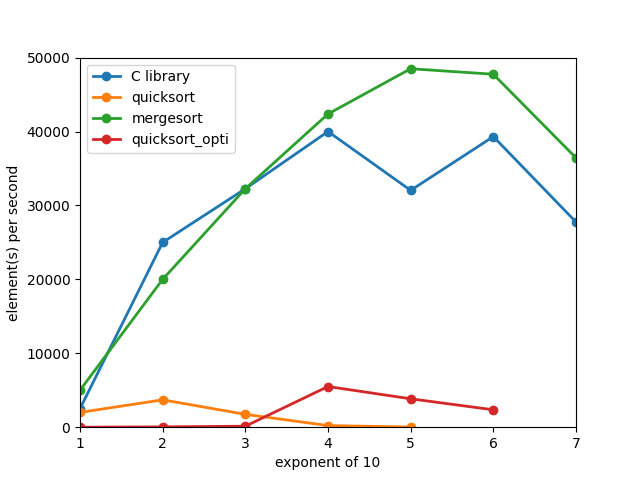
\includegraphics[width=0.8\textwidth]{ori.up.csvtime.png}
		\caption{performance under ascending sequence}
		\label{}
	\end{figure}
	\subsubsection{performance under descending sequence }
	\begin{figure}[H]
		\centering
		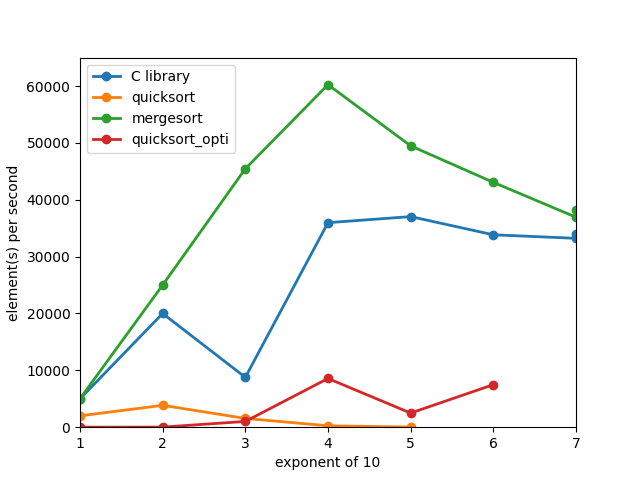
\includegraphics[width=0.8\textwidth]{ori.down.csvtime.png}
		\caption{performance under descending sequence}
		\label{}
	\end{figure}
	No matter the array is descending sequence or ascending sequence,both of these two figures goes so similar.The quicksort becomes the slowest one and even can't work appropriately when the length of array goes larger than $10^5$.Our optimized one seems to be better but just a little bit and can't work when the array goes too big.But merge sort works very well,even better than the standard library,interesting.
	\subsection{memory consumption analysis}
	\subsubsection{quicksort}
	Since C language is complied by the compiler into the machine code,we cannot measure the memory consumption of several codes inner the program.And measure the whole memory consumption is meaningless since the size of the array will take the biggest part.Thus,we might can try to trace the depth of the recursion and thus infer the memory consumption.
	I declared a global variable $deepStack$ to store the length of the array.And due to C language do not provide array method like push and pop,we use a global variable $deepStackPointer$ to stimulate the current pointer.Before the call of sort,we init a variable and pass the pointer into the recursion.Here is a example when the input is perfectly random and the length is $10^6$.
	\begin{figure}[H]
		\centering
		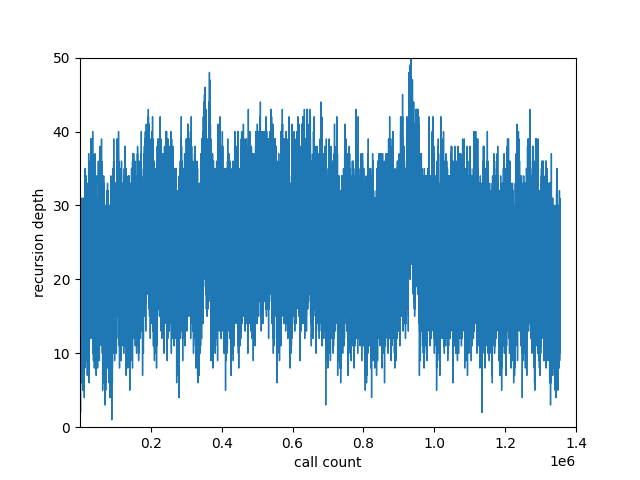
\includegraphics[width=0.8\textwidth]{stack.png}
		\caption{the recursion depth of quicksort}
		\label{10}
	\end{figure}
	As you can see,the recursion depth is under 50 in most cases,and memory consumption will not exceed 50*$p$*sizeof(double) bits,where $p$ is the number variables used in each function call,about 10 maybe.So the memory consumption will not exceed 4kb,which is not too much.
	
	However,what about the extreme case,like the array is completely in ascending sequence?

	That will make the recursion depth to be as deep as the length of the array,since the recursion will goes very deep in only one side,which is might the reason of stack overflow.
	\subsubsection{merge sort}
	From the given code,we can easily find the merge sort rely on a space as large as the origin array.So the memory consumption will not be small but very stable.
\section{Optimization}
	\subsection{quicksort}
	The given quicksort algorithm made a significant mistake that it didn't exchange the pivot element with a random element,which might cause the worst case performance at some extreme cases(such as array is a ascending sequence).Thus,our optimization is enable the omp parallel and use the random function to exchange the pivot element with a random element.

\end{document}
